% Options for packages loaded elsewhere
\PassOptionsToPackage{unicode}{hyperref}
\PassOptionsToPackage{hyphens}{url}
%
\documentclass[
]{article}
\usepackage{amsmath,amssymb}
\usepackage{lmodern}
\usepackage{iftex}
\ifPDFTeX
  \usepackage[T1]{fontenc}
  \usepackage[utf8]{inputenc}
  \usepackage{textcomp} % provide euro and other symbols
\else % if luatex or xetex
  \usepackage{unicode-math}
  \defaultfontfeatures{Scale=MatchLowercase}
  \defaultfontfeatures[\rmfamily]{Ligatures=TeX,Scale=1}
\fi
% Use upquote if available, for straight quotes in verbatim environments
\IfFileExists{upquote.sty}{\usepackage{upquote}}{}
\IfFileExists{microtype.sty}{% use microtype if available
  \usepackage[]{microtype}
  \UseMicrotypeSet[protrusion]{basicmath} % disable protrusion for tt fonts
}{}
\makeatletter
\@ifundefined{KOMAClassName}{% if non-KOMA class
  \IfFileExists{parskip.sty}{%
    \usepackage{parskip}
  }{% else
    \setlength{\parindent}{0pt}
    \setlength{\parskip}{6pt plus 2pt minus 1pt}}
}{% if KOMA class
  \KOMAoptions{parskip=half}}
\makeatother
\usepackage{xcolor}
\IfFileExists{xurl.sty}{\usepackage{xurl}}{} % add URL line breaks if available
\IfFileExists{bookmark.sty}{\usepackage{bookmark}}{\usepackage{hyperref}}
\hypersetup{
  pdftitle={Assessing the impact of nonverbal communication cues in online teaching},
  pdfauthor={Maria Osipenko, Kathrin Heller},
  hidelinks,
  pdfcreator={LaTeX via pandoc}}
\urlstyle{same} % disable monospaced font for URLs
\usepackage[margin=1in]{geometry}
\usepackage{longtable,booktabs,array}
\usepackage{calc} % for calculating minipage widths
% Correct order of tables after \paragraph or \subparagraph
\usepackage{etoolbox}
\makeatletter
\patchcmd\longtable{\par}{\if@noskipsec\mbox{}\fi\par}{}{}
\makeatother
% Allow footnotes in longtable head/foot
\IfFileExists{footnotehyper.sty}{\usepackage{footnotehyper}}{\usepackage{footnote}}
\makesavenoteenv{longtable}
\usepackage{graphicx}
\makeatletter
\def\maxwidth{\ifdim\Gin@nat@width>\linewidth\linewidth\else\Gin@nat@width\fi}
\def\maxheight{\ifdim\Gin@nat@height>\textheight\textheight\else\Gin@nat@height\fi}
\makeatother
% Scale images if necessary, so that they will not overflow the page
% margins by default, and it is still possible to overwrite the defaults
% using explicit options in \includegraphics[width, height, ...]{}
\setkeys{Gin}{width=\maxwidth,height=\maxheight,keepaspectratio}
% Set default figure placement to htbp
\makeatletter
\def\fps@figure{htbp}
\makeatother
\setlength{\emergencystretch}{3em} % prevent overfull lines
\providecommand{\tightlist}{%
  \setlength{\itemsep}{0pt}\setlength{\parskip}{0pt}}
\setcounter{secnumdepth}{5}
\newlength{\cslhangindent}
\setlength{\cslhangindent}{1.5em}
\newlength{\csllabelwidth}
\setlength{\csllabelwidth}{3em}
\newlength{\cslentryspacingunit} % times entry-spacing
\setlength{\cslentryspacingunit}{\parskip}
\newenvironment{CSLReferences}[2] % #1 hanging-ident, #2 entry spacing
 {% don't indent paragraphs
  \setlength{\parindent}{0pt}
  % turn on hanging indent if param 1 is 1
  \ifodd #1
  \let\oldpar\par
  \def\par{\hangindent=\cslhangindent\oldpar}
  \fi
  % set entry spacing
  \setlength{\parskip}{#2\cslentryspacingunit}
 }%
 {}
\usepackage{calc}
\newcommand{\CSLBlock}[1]{#1\hfill\break}
\newcommand{\CSLLeftMargin}[1]{\parbox[t]{\csllabelwidth}{#1}}
\newcommand{\CSLRightInline}[1]{\parbox[t]{\linewidth - \csllabelwidth}{#1}\break}
\newcommand{\CSLIndent}[1]{\hspace{\cslhangindent}#1}
\usepackage{booktabs}
\usepackage{longtable}
\usepackage{array}
\usepackage{multirow}
\usepackage{wrapfig}
\usepackage{float}
\usepackage{colortbl}
\usepackage{pdflscape}
\usepackage{tabu}
\usepackage{threeparttable}
\usepackage{threeparttablex}
\usepackage[normalem]{ulem}
\usepackage{makecell}
\usepackage{xcolor}
\ifLuaTeX
  \usepackage{selnolig}  % disable illegal ligatures
\fi

\title{Assessing the impact of nonverbal communication cues in online teaching}
\author{Maria Osipenko, Kathrin Heller}
\date{}

\begin{document}
\maketitle

\hypertarget{introduction}{%
\section{Introduction}\label{introduction}}

\hypertarget{research-question}{%
\subsection{Research question}\label{research-question}}

Do different usage patterns of nonverbal communication cues of course instructor as colors, markers, paintings have impact on learning success in online format?

For previous research see Ng and Przybylek (2021), Dixson et al. (2016), Cheng et al. (2014), and Tawil (2019).

\hypertarget{retrospective-feature-extraction}{%
\subsection{Retrospective feature extraction}\label{retrospective-feature-extraction}}

We extract features retrospectively from lecture notes of three semesters and two courses on statistics.

\begin{figure}

{\centering 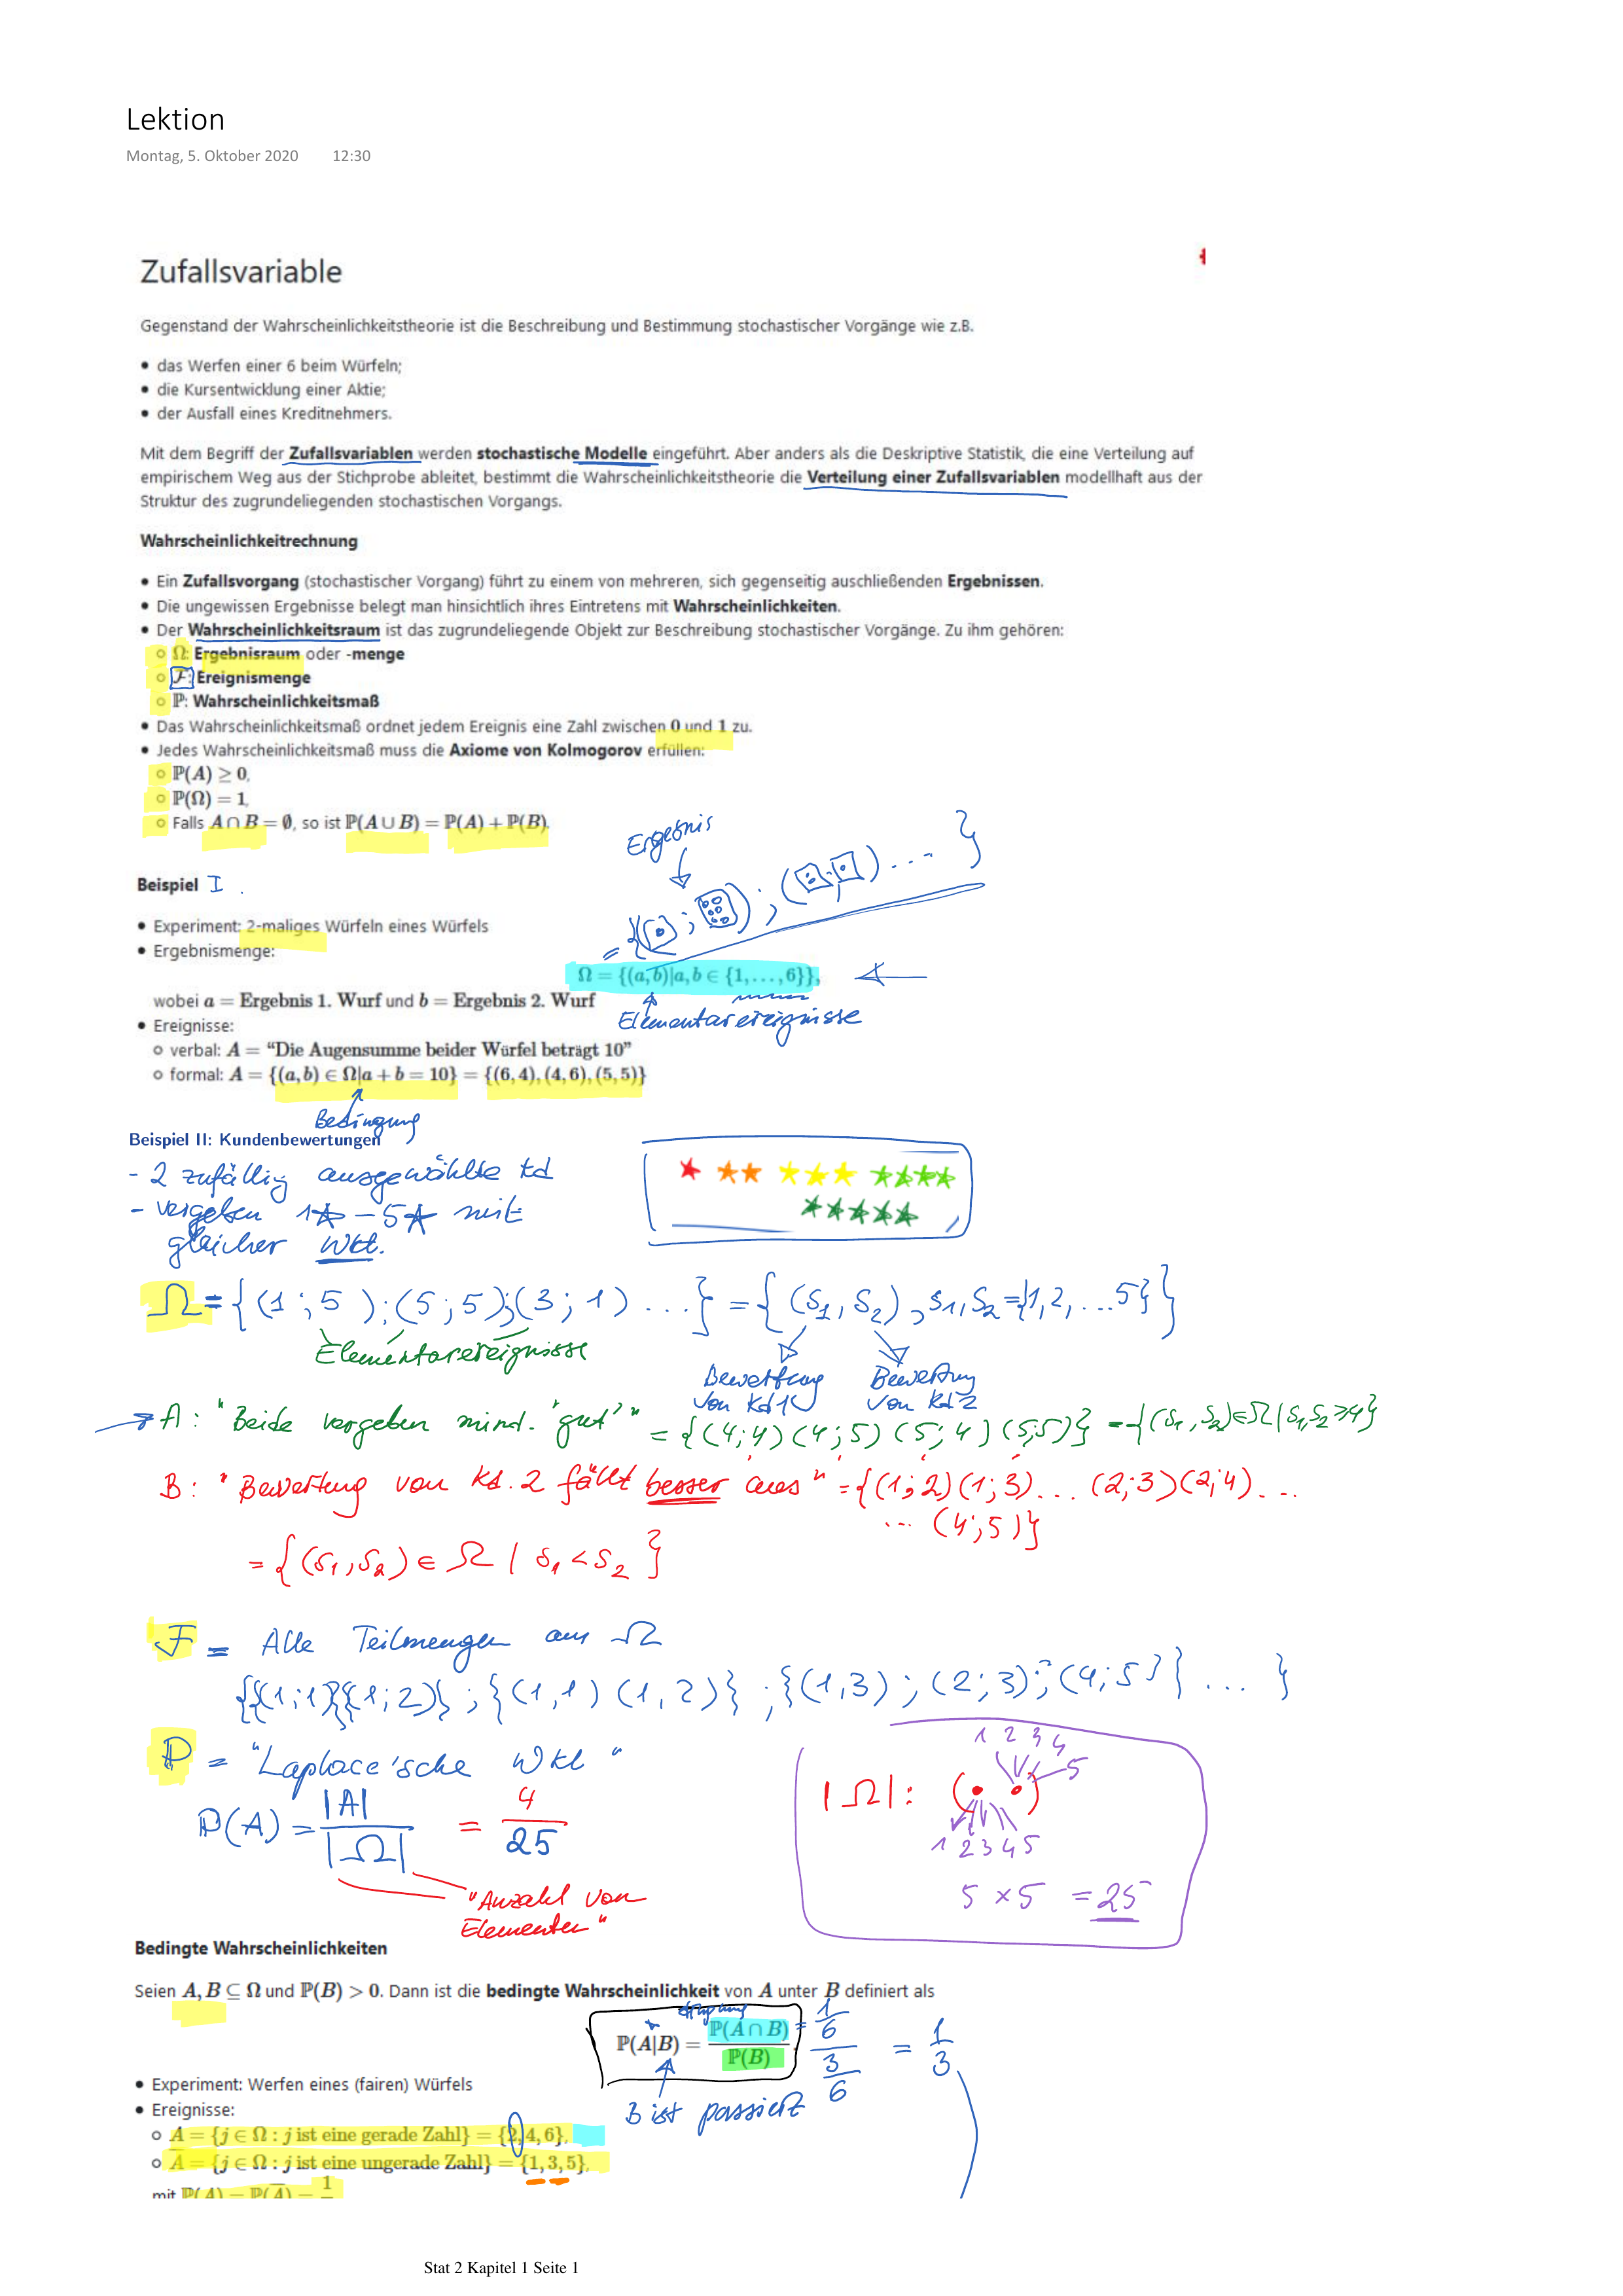
\includegraphics[width=0.25\linewidth]{paper_files/figure-latex/figPage-1} 

}

\caption{An example of lecture notes}\label{fig:figPage}
\end{figure}

\hypertarget{documentation-of-the-data-aquisition-process}{%
\subsection{Documentation of the data aquisition process}\label{documentation-of-the-data-aquisition-process}}

\hypertarget{results}{%
\section{Results}\label{results}}

A table:

see our results in Table \ref{tab:table00}

\begin{table}

\caption{\label{tab:table00}Description of the final textual corpus}
\centering
\begin{tabular}[t]{l|l|l}
\hline
Year & News Articles (merged) & Average Word Count\\
\hline
2015 & 4,395 & 823\\
\hline
2016 & 5,391 & 840\\
\hline
2017 & 5,738 & 923\\
\hline
2018 & 8,465 & 1,352\\
\hline
2019 & 6,435 & 1,401\\
\hline
All years & 30,424 & 1,114\\
\hline
\end{tabular}
\end{table}

\hypertarget{literature}{%
\section*{Literature}\label{literature}}
\addcontentsline{toc}{section}{Literature}

\hypertarget{refs}{}
\begin{CSLReferences}{1}{0}
\leavevmode\vadjust pre{\hypertarget{ref-cheng2014}{}}%
Cheng, Dong Seon, Hugues Salamin, Pietro Salvagnini, Marco Cristani, Alessandro Vinciarelli, and Vittorio Murino. 2014. {``Predicting Online Lecture Ratings Based on Gesturing and Vocal Behavior.''} \emph{J Multimodal User Interfaces} 8 (June): 151--60. \url{https://doi.org/10.1007/s12193-013-0142-z}.

\leavevmode\vadjust pre{\hypertarget{ref-dixson2016}{}}%
Dixson, Marcia, Mackenzie Greenwell, Christie Rogers-Stacy, Tyson Weister, and Sara Lauer. 2016. {``Nonverbal Immediacy Behaviors and Online Student Engagement: Bringing Past Instructional Research into the Present Virtual Classroom.''} \emph{Communication Education} 66 (August): 1--17. \url{https://doi.org/10.1080/03634523.2016.1209222}.

\leavevmode\vadjust pre{\hypertarget{ref-ng2021}{}}%
Ng, Yen, and Adam Przybylek. 2021. {``Instructor Presence in Video Lectures: Preliminary Findings from an Online Experiment.''} \emph{IEEE Access} 9 (March): 36485--99. \url{https://doi.org/10.1109/ACCESS.2021.3058735}.

\leavevmode\vadjust pre{\hypertarget{ref-tawil2019}{}}%
Tawil, Rima. 2019. {``Nonverbal Communication in Text-Based, Asynchronous Online Education.''} \emph{International Review of Research in Open and Distance Learning} 20 (February): 145--64. \url{https://doi.org/10.19173/irrodl.v20i1.3705}.

\end{CSLReferences}

\end{document}
